\documentclass[conference]{IEEEtran}
\IEEEoverridecommandlockouts
% The preceding line is only needed to identify funding in the first footnote. If that is unneeded, please comment it out.
\usepackage{cite}
\usepackage{amsmath,amssymb,amsfonts}
\usepackage{algorithmic}
\usepackage{graphicx}
\usepackage{textcomp}
\usepackage{xcolor}
\usepackage{subcaption}

\def\BibTeX{{\rm B\kern-.05em{\sc i\kern-.025em b}\kern-.08em
    T\kern-.1667em\lower.7ex\hbox{E}\kern-.125emX}}
\begin{document}

\title{Free3D - Free-viewpoint 3D video creation}

\author{\IEEEauthorblockN{Felix Brunn}
\IEEEauthorblockA{\textit{Faculty Digital Media} \\
\textit{Hochschule Furtwangen University}\\
Furtwangen, Germany \\
lix.brunn@gmail.com}
\and
\IEEEauthorblockN{Jan Christmeier}
\IEEEauthorblockA{\textit{Faculty Digital Media} \\
\textit{Hochschule Furtwangen University}\\
Furtwangen, Germany \\
jan97@kabelmail.de}
\and
\IEEEauthorblockN{Nick P.  H{\"a}cker}
\IEEEauthorblockA{\textit{Faculty Digital Media} \\
\textit{Hochschule Furtwangen University}\\
Furtwangen, Germany \\
nick.athaeck@gmail.com}
\and
\IEEEauthorblockN{Laura C. Stempfle}
\IEEEauthorblockA{\textit{Faculty Digital Media} \\
\textit{Hochschule Furtwangen University}\\
Furtwangen, Germany \\
laurastempfle@gmx.net}
\and
\IEEEauthorblockN{Lukas Willmann}
\IEEEauthorblockA{\textit{Faculty Digital Media} \\
\textit{Hochschule Furtwangen University}\\
Furtwangen, Germany \\
lwi45898@stud.hs-furtwangen.de}
\and
\IEEEauthorblockN{Simon Zakowski}
\IEEEauthorblockA{\textit{Faculty Digital Media} \\
\textit{Hochschule Furtwangen University}\\
Furtwangen, Germany \\
sza45046@stud.hs-furtwangen.de}
\and
\IEEEauthorblockN{Prof. Dr. Uwe Hahne}
\IEEEauthorblockA{\textit{Faculty Digital Media} \\
\textit{Hochschule Furtwangen University}\\
Furtwangen, Germany \\
uwe.hahne@hs-furtwangen.de}

}

\maketitle

\begin{abstract}
This student research project explores the recording of full three-dimensional (3D) scenes using only three Azure Kinect cameras. By leveraging novel methodologies such as Neural Radiance Fields (NeRF) and 3D Gaussian Splatting, the captured images are processed into a "4D data structure", enabling the creation of new videos from any perspective. The project's goal is to determine the extent to which visually high-quality 3D scenes can be generated with minimal equipment. The study highlights the potential of these advanced techniques to enhance for example online learning experiences by providing an accessible tool for creating immersive 3D content. Experiments demonstrated that using depth data from RGB-D cameras compensates for the reduced number of input images, maintaining high visual quality. The results show that combining static Gaussian Splatting-generated backgrounds with point cloud data from Azure Kinect cameras can produce impressive 3D scene reconstructions with reduced computational demands, making the technology more accessible and cost-effective.
\end{abstract}

\begin{IEEEkeywords}
NeRF, Gaussian Splatting, Volumetric Video, Point Cloud, Azure Kinect
\end{IEEEkeywords}

\section{Introduction}
This student research project from our university is
about recording a full three-dimensional (3D) scene using only three Azure Kinect 3D cameras. The utilization of novel methodologies, such as Neural Radiance Fields (NeRF) and 3D Gaussian Splatting, enables the saving and processing of the recorded images in a novel 4D data structure, thereby facilitating the generation of new videos of the scene from any novel perspective. The research project sought to ascertain the extent to which visually high-quality 3D images can be generated using simple means and a small number of cameras. To this end, current research work was reproduced and
combined in order to generate new perspectives from the self-recorded data. 

\subsection{Motivation}
While the world is 3D, most existing visualization methods work only in 2D. A field suffering from this loss of information due to the dimension reduction is
higher education. Complex machines and concepts require intensive training of all aspects to be mastered. The objective of this project is to provide access to this missing information in a lightweight, easily accessible application. Therefore, the application should be able to replay dynamic real-world scenes in order to be explored by learners. Unlike traditional methods that require a lot of cameras, we use only three Azure Kinect cameras and utilize novel view synthesis methods, reducing both setup complexity and cost. We investigate the effectiveness of NeRF and Gaussian Splatting techniques for reconstructing 3D
scenes, and aim to enhance online learning experiences by providing educators with an accessible tool set for creating immersive 3D content.

\section{Related Work}
Since NeRF \cite{b4} provided revolutionary results on novel view synthesis, the topic has skyrocketed.
Many thousand papers building on the foundation
of the original NeRF were published since 2020 that
improved several aspects of NeRF or sought different approaches. In our project, we tried to cluster various approaches and examined to what extent Im4D \cite{b3}, 4K4D \cite{b5} or Dynamic
3D Gaussians \cite{b2} are suitable for our setup
with a strongly reduced number of cameras as input.
Im4D \cite{b3} is a hybrid scene representation combining the consistent rendering of grid-based methods with the appearance representation of multi-view image-based methods. In their work the dynamic geometry is encoded as a 4D density function made of
spatio-temporal feature planes and a small MLP network. Detailed appearances are not memorized but inferred from image features. Im4D achieves state-of-the art rendering quality and performance while realizing
real-time rendering on a single GPU. 
4K4D \cite{b5} is an extension of the Im4D paper, in which realistic
real-time synthesis of dynamic 3D scenes with 4k resolution can be displayed. The speed of high-resolution
images is still limited. To solve this problem, the points
are regulated and robustly optimized in a natural way
based on a 4D feature grid. In addition, a novel hybrid
appearance model is used, which significantly increases
rendering quality while maintaining efficiency.
In addition to NeRF, there are other options such
as 3D Gaussian Splatting \cite{b1} to reconstruct a
3D scene from images. While the original approach (Gaussian Splatting) is
also only suitable for static images, Dynamic 3D Gaussians \cite{b2} presents a method for dynamic scene
synthesis and dense 6-DOF tracking, using an analysis-by-synthesis framework with 3D Gaussians. The dynamic scenes are modeled by allowing Gaussians to
move and rotate over time with constraints to ensure
physical accuracy. This approach eliminates the need
for correspondence or flow input, enabling applications
such as first-person view synthesis, dynamic scene composition, and 4D video editing.

\section{Method}
\subsection{Recording Setup}
\begin{figure}[h]
    \centering
    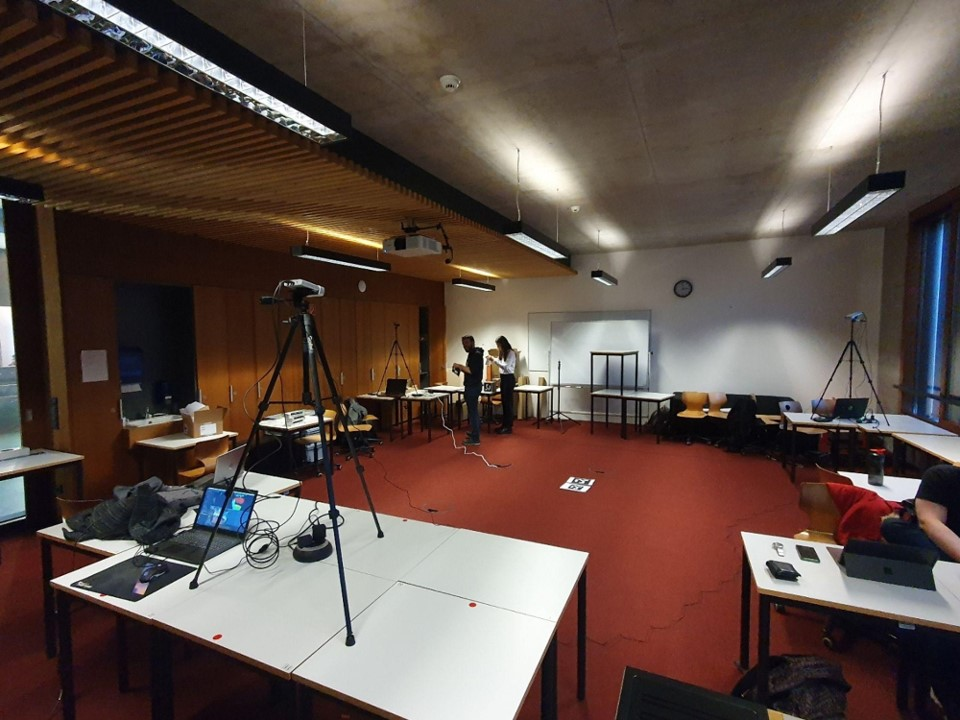
\includegraphics[width=1.0\linewidth]{Pictures/Aufbau.jpg}
    \caption{Simple Setup for Recordings}
    \label{Simple set-up for Recordings}
\end{figure}
We tried to use as little material as possible for our multi-view camera setup. We used three Azure Kinect cameras. To minimize frame loss, one laptop was connected to each camera. MKV files were recorded via the Recording.exe of the Azure Kinect SDK. The recordings were made at a resolution of the RBG camera of 1920x1080 pixels, a frame rate of 30 frames per second and a length of ten seconds. The depth sensor was set to “NFOV\_2X2BINNED” mode.

The procedure was as follows. First, a ten-second recording of the calibration object was made (see chapter on marker-based calibration). This recording can be used to determine the positions of the cameras. After this calibration recording, the cameras must no longer be moved. Once the calibration object has been recorded, various recordings can be made on this basis. As soon as the cameras have been moved, a new calibration image must be taken.
As soon as the images are available, the point clouds can be generated with the software of our project, which can later be combined with static Gaussian Splats.

The cameras were set up at a distance of 1.5 meters to 3.5 meters from the calibration object. The tripods on which the cameras were placed had a height of approx. 1.80 meters. The cameras were positioned at an angle of approx. 120 degrees to each other.


\begin{figure}[h]
    \centering
    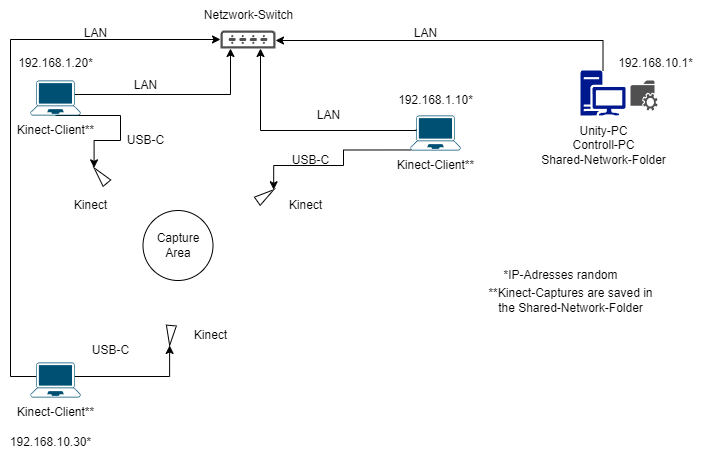
\includegraphics[width=1.0\linewidth]{Pictures/physical-infrastructure.png}
    \caption{Physical Setup with network infrastructure}
    \label{physical_setup}
\end{figure}

A network structure (see Fig. \ref{physical_setup}) has been set up to reduce the physical workload and minimize the number of personnel required to start a recording. The other laptops can be controlled for recording via a web app and a socket connection (see Fig. \ref{Hirachy}). The network also makes it possible for the files to be directly available on the computer on which work is to continue.

\begin{figure}[h]
    \centering
    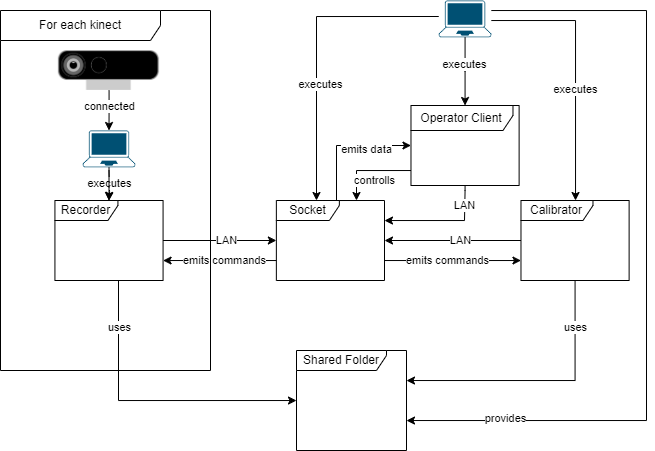
\includegraphics[width=1.0\linewidth]{Pictures/Hierachy.drawio.png}
    \caption{Connection of a PC with Kinect and software structure}
    \label{Hirachy}
\end{figure}

\subsection{Marker Based Calibrating}
To ensure a simple setup, camera calibration via marker tracking was applied. The open source project OpenCV has provided us with the basis for this. An ArUco marker object and a ChArUco poster were used as markers.
\subsubsection{ArUco Marker}
\begin{figure}[h]
    \centering
    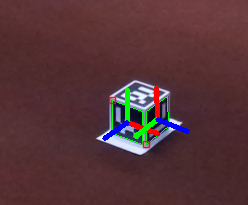
\includegraphics[width=1.0\linewidth]{Pictures/TrackedMarkers.png}
    \caption{Tracked ArUco Marker (30 and 1)}
    \label{Tracked ArUco Marker (30 and 1)}
\end{figure}
An ArUco marker object was created as a cube with one marker on each side. The markers have different IDs. The cube has an edge length of 17 cm x 17 cm x 17 cm. Based on the tracked markers in the camera images (see Fig. \ref{Tracked ArUco Marker (30 and 1)}), the center of the cube can be calculated, which is then set as the center of the scene and can be used to determine the camera positions and orientations. Due to the size of the marker and the incidence of light in the scene, inaccuracies may occur when tracking the markers in the camera image. During the recording in which the camera positions are determined, ten seconds are recorded. With 30 frames per second, 300 different results of orientation matrix and position vector per marker ID can be calculated. To analyse the position of the camera, an algorithm has been developed that compares pairs of detected marker positions. This comparison results in a small difference in the cube position. Once the relevant pairs have been determined, the median of these pairing results is used to determine the camera position in relation to the cube position.

\subsubsection{ChArUco-Board}
\begin{figure}[h]
    \centering
    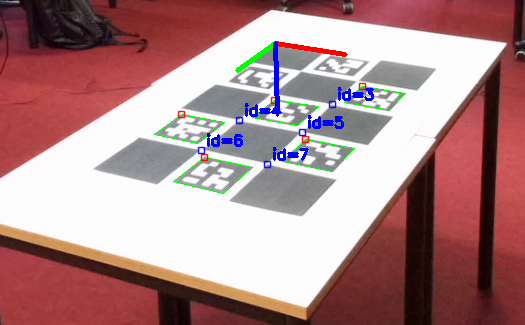
\includegraphics[width=1.0\linewidth]{Pictures/TrackedMarkers_Charuco.png}
    \caption{Tracked ChArUco-Board}
    \label{Tracked ChArUco-Board}
\end{figure}
A ChArUco board was created next to the ArUco Cube. This is printed on an A1 poster. The ArUco markers on it have a size of 11.2 cm x 11.2 cm and the chessboard surfaces have a size of 15 cm x 15 cm.

Again, 300 different orientation matrices and position vectors can be calculated with a calibration video of ten seconds. However, only one position is output by OpenCV. Accordingly, the median of the calculated results can be taken and used as the position of the poster. This can be used to determine the position of the camera.

\subsection{Point cloud post-processing}
\begin{figure}[h]
    \begin{subfigure}{.24\textwidth}
    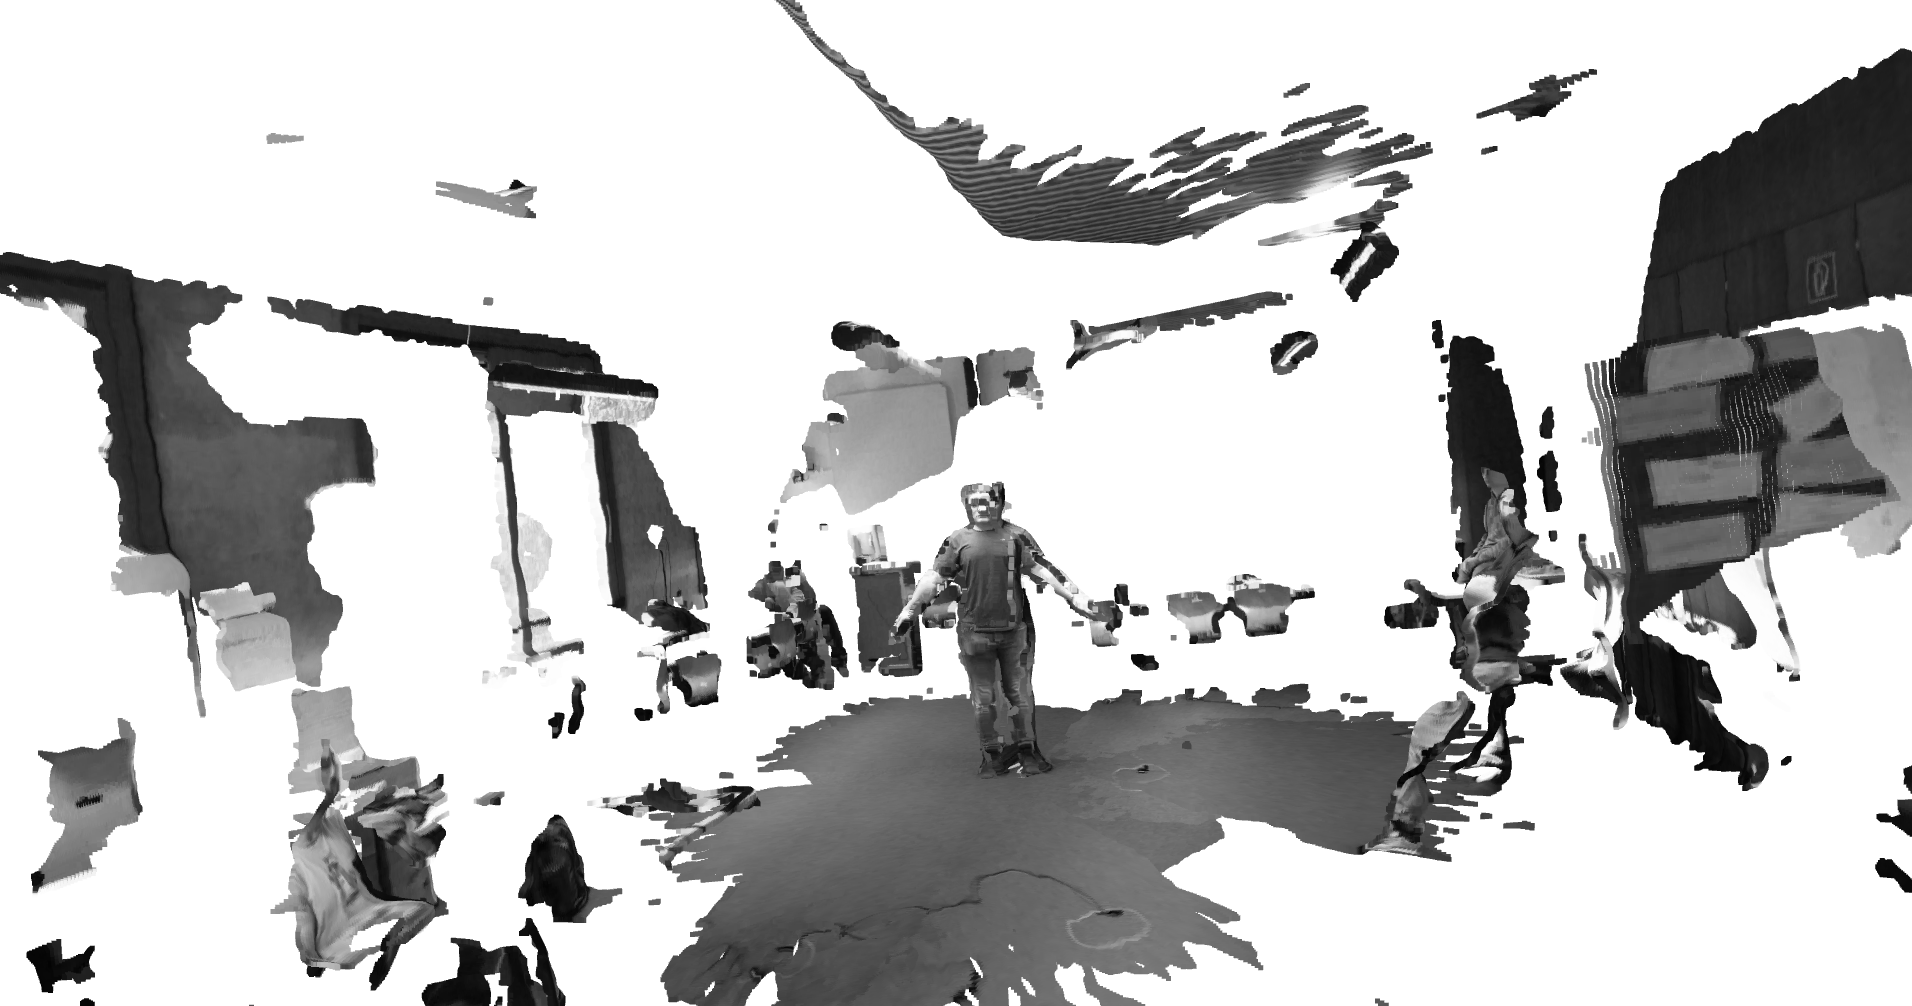
\includegraphics[width=\linewidth]{Pictures/Pointcloud_Kinects.png}
    \end{subfigure}
    \begin{subfigure}{.24\textwidth}
    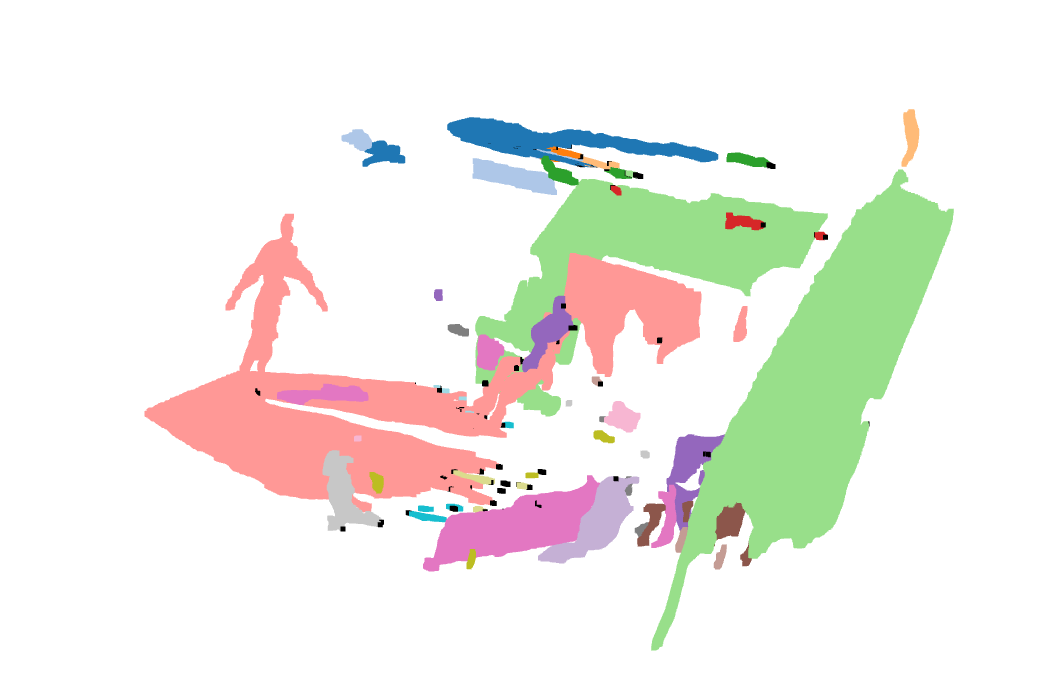
\includegraphics[width=\linewidth]{Pictures/DB_Scan.png}
    \end{subfigure}
    \begin{subfigure}{.24\textwidth}
    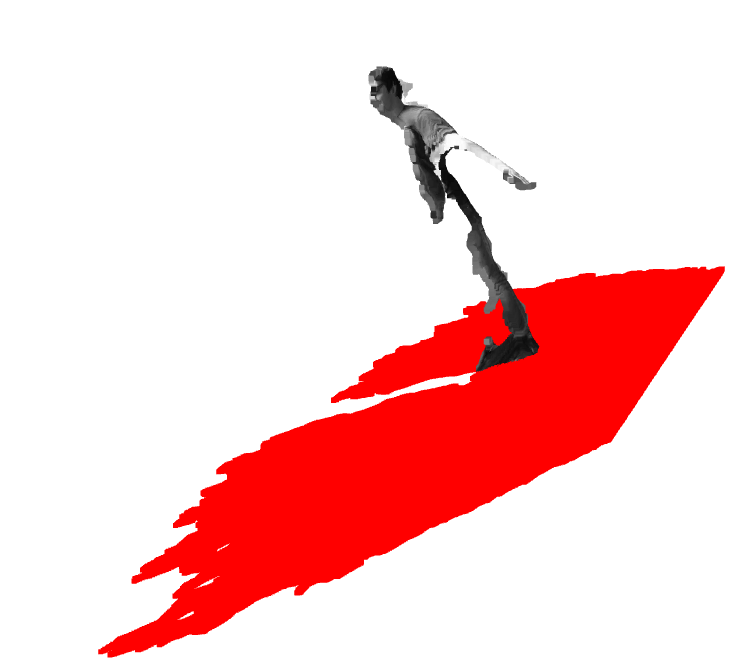
\includegraphics[width=\linewidth]{Pictures/PlaneSegmentation.png}
    \end{subfigure}
    \begin{subfigure}{.24\textwidth}
    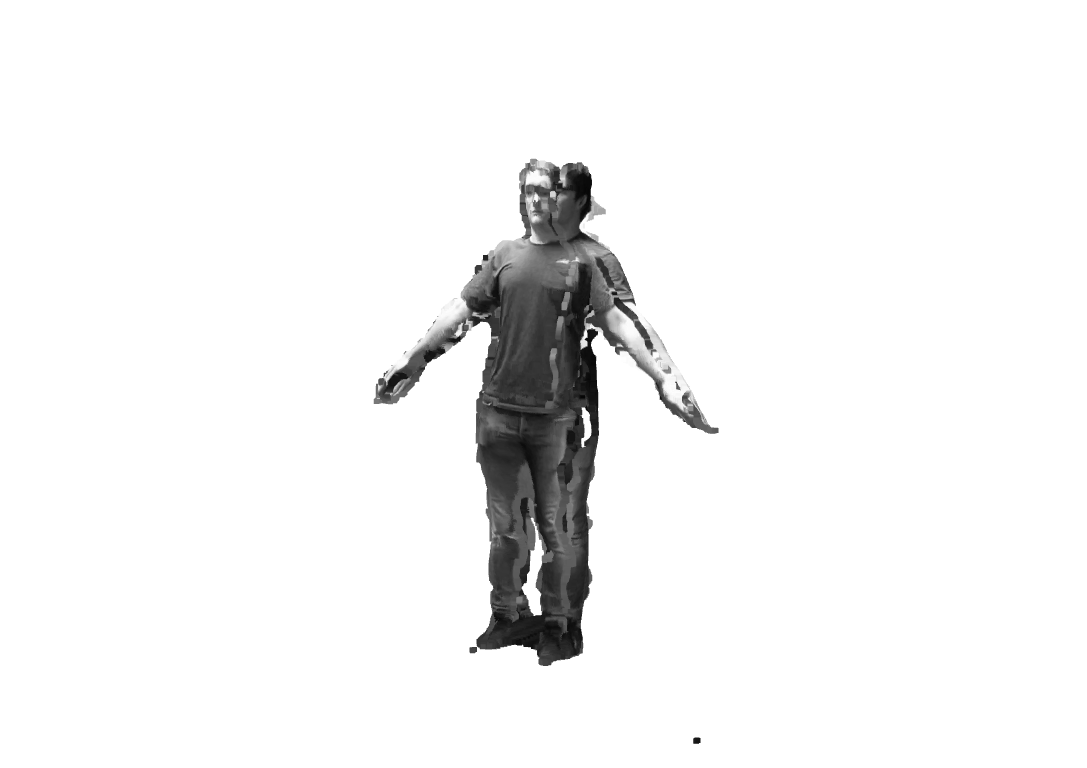
\includegraphics[width=\linewidth]{Pictures/ExtractetObjectInCenter.png}
    \end{subfigure}
    \caption{Post-processing from whole room to extracted center}
    \label{fig:Post-processing}
\end{figure}
Once the cameras have been calibrated, the point cloud can be generated. Open3D was used for this. The RGB-D data was extracted from the MKV files and calculated with the calibration data so that the data can be combined to form a point cloud. Open3D functions were used to extract the object or person in the center (see Fig. \ref{fig:Post-processing}). DB-Scan can be used to select the cluster with the most points. This is usually the cluster with the desired object.

The ground can be removed from the scene with a surface selection function.

Once these functions have been carried out, the object in the scene is released. However, this is subject to errors depending on the scene. See results for more information.

\subsection{Testing of various existing scientific papers}

\begin{figure}[h]
    \centering
    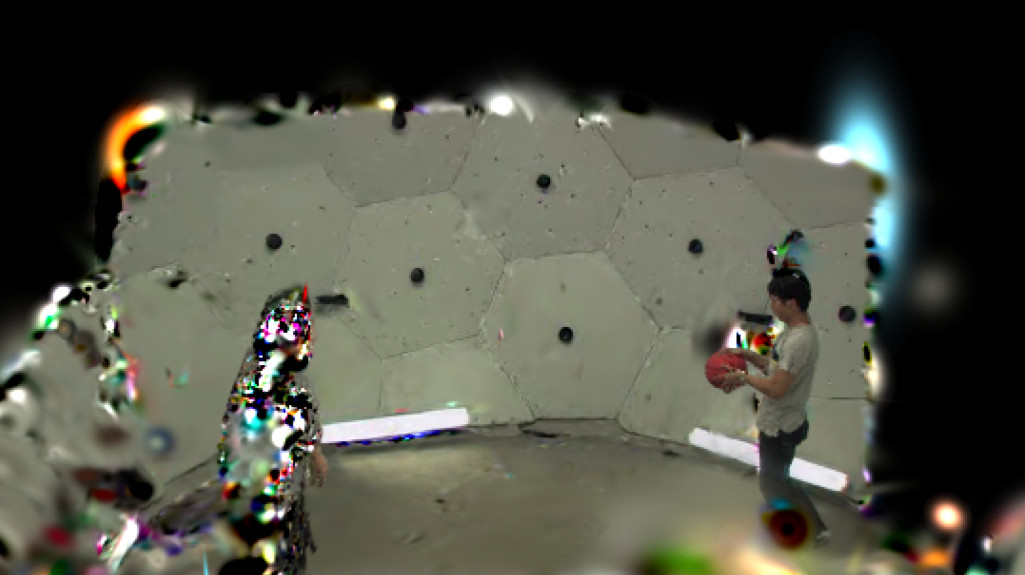
\includegraphics[width=1.0\linewidth]{Pictures/dgs_3Cams.jpg}
    \caption{Generating dynamic Gaussian Splats with only 3 Perspectives}
    \label{dgs_3cams}
\end{figure}

Among others, nerfstudio \cite{b6} and DUSt3R \cite{b7} were tested to create the static scene. Static NeRFs and Gaussian Splats could be generated with nerfstudio. These Gaussian Splats could be easily inserted into Unity using an existing plugin.
With DUSt3R, meshes could also be created with only three images of the Kinect structure. Compared to the Gaussian Splats and NeRFs from nerfstudio, however, these were visually less convincing.

To visualize the dynamic elements in the scene, Im4D, 4K4D and Dynamic Gaussian Spaltting were considered. After 4K4D was published as new research following Im4D, Im4D was neglected.
4K4D could be made to work with the published tools, but there were problems transferring this method to our data. When trying to process only 3 camera perspectives in the project, 4K4D could not be executed.

Dynamic Gaussian Splatting could be executed. With the data provided by Luiten et. al. only three perspectives could be selected and the project executed (see Fig. \ref{dgs_3cams}). As expected, the visual result was significantly worse than with more perspectives. However, the scene could be recognized. Due to time constraints, we were unable to carry out any further detailed tests with our data using the Dynamic Gaussian Splatting project as part of our project.

\subsection{Combining point clouds and Gaussian Splats}
To display the point clouds, we decided to visualise them using Unity. We were able to use a Gaussian Splat integration in Unity that allows us to visualise a Gaussian Splat when given a PLY file. We wrote our own plugin to animate our point clouds and display them in Unity. Fig. \ref{fig:ResultPictures} shows the results of our successful combination. You can see the typical appearance of a Gaussian splat, combined with our point cloud in the center.
\section{Results}
\begin{figure}[h]
    \begin{subfigure}{.24\textwidth}
    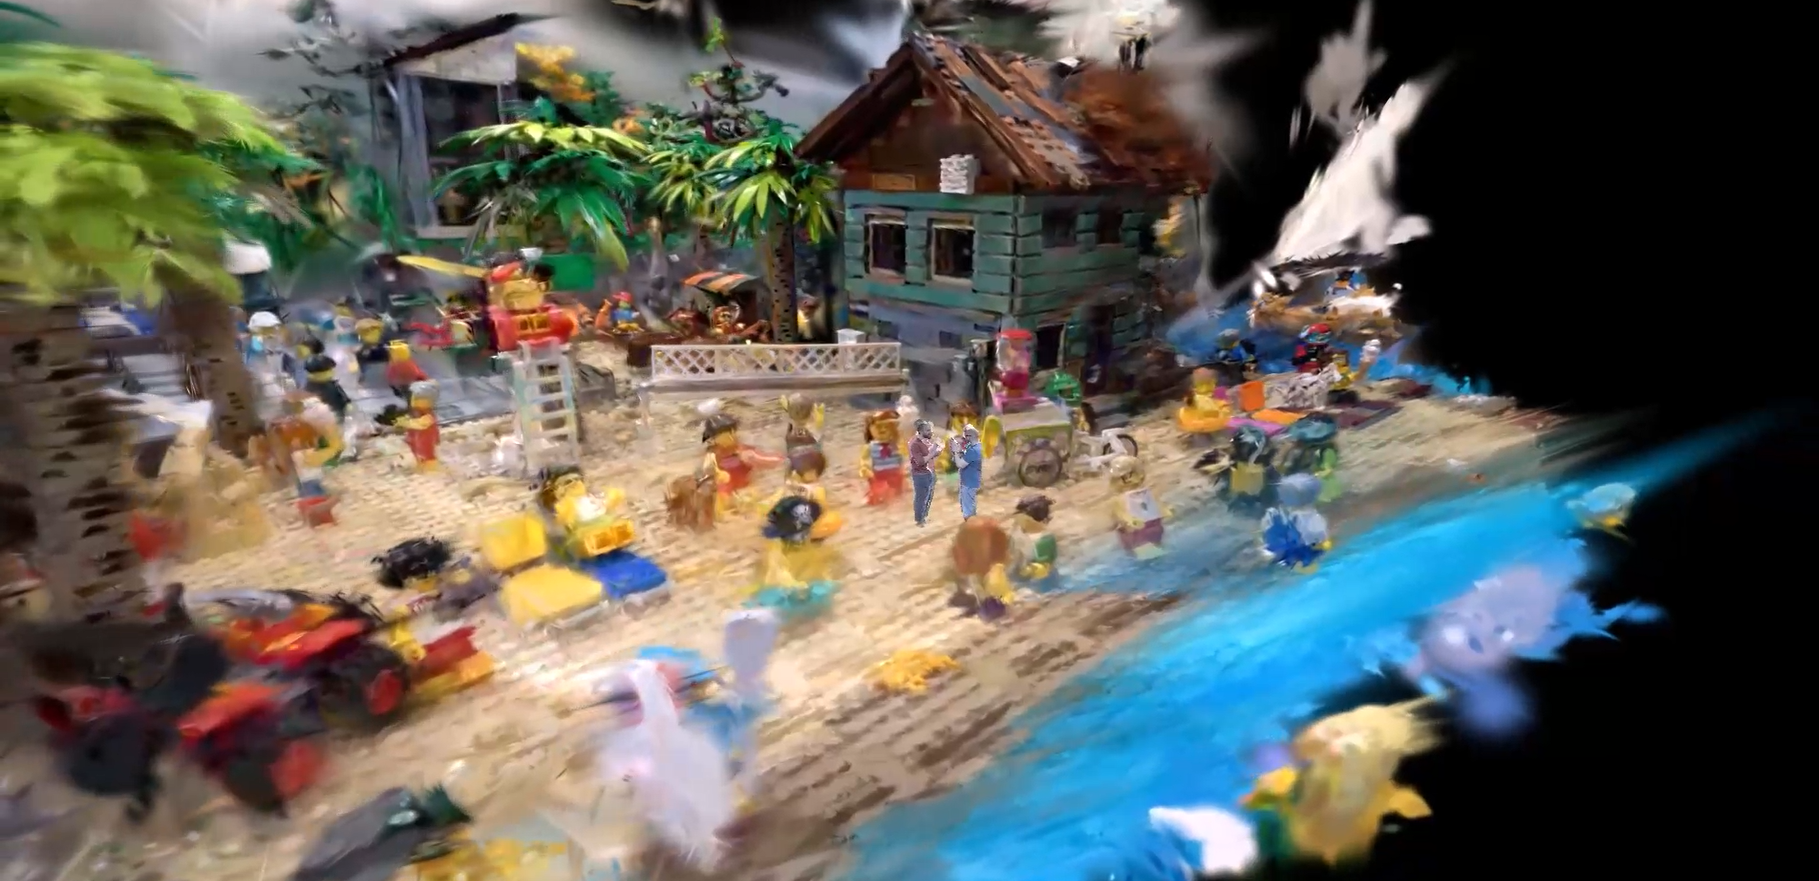
\includegraphics[width=\linewidth]{Pictures/ResPic1.png}
    \end{subfigure}
    \begin{subfigure}{.24\textwidth}
    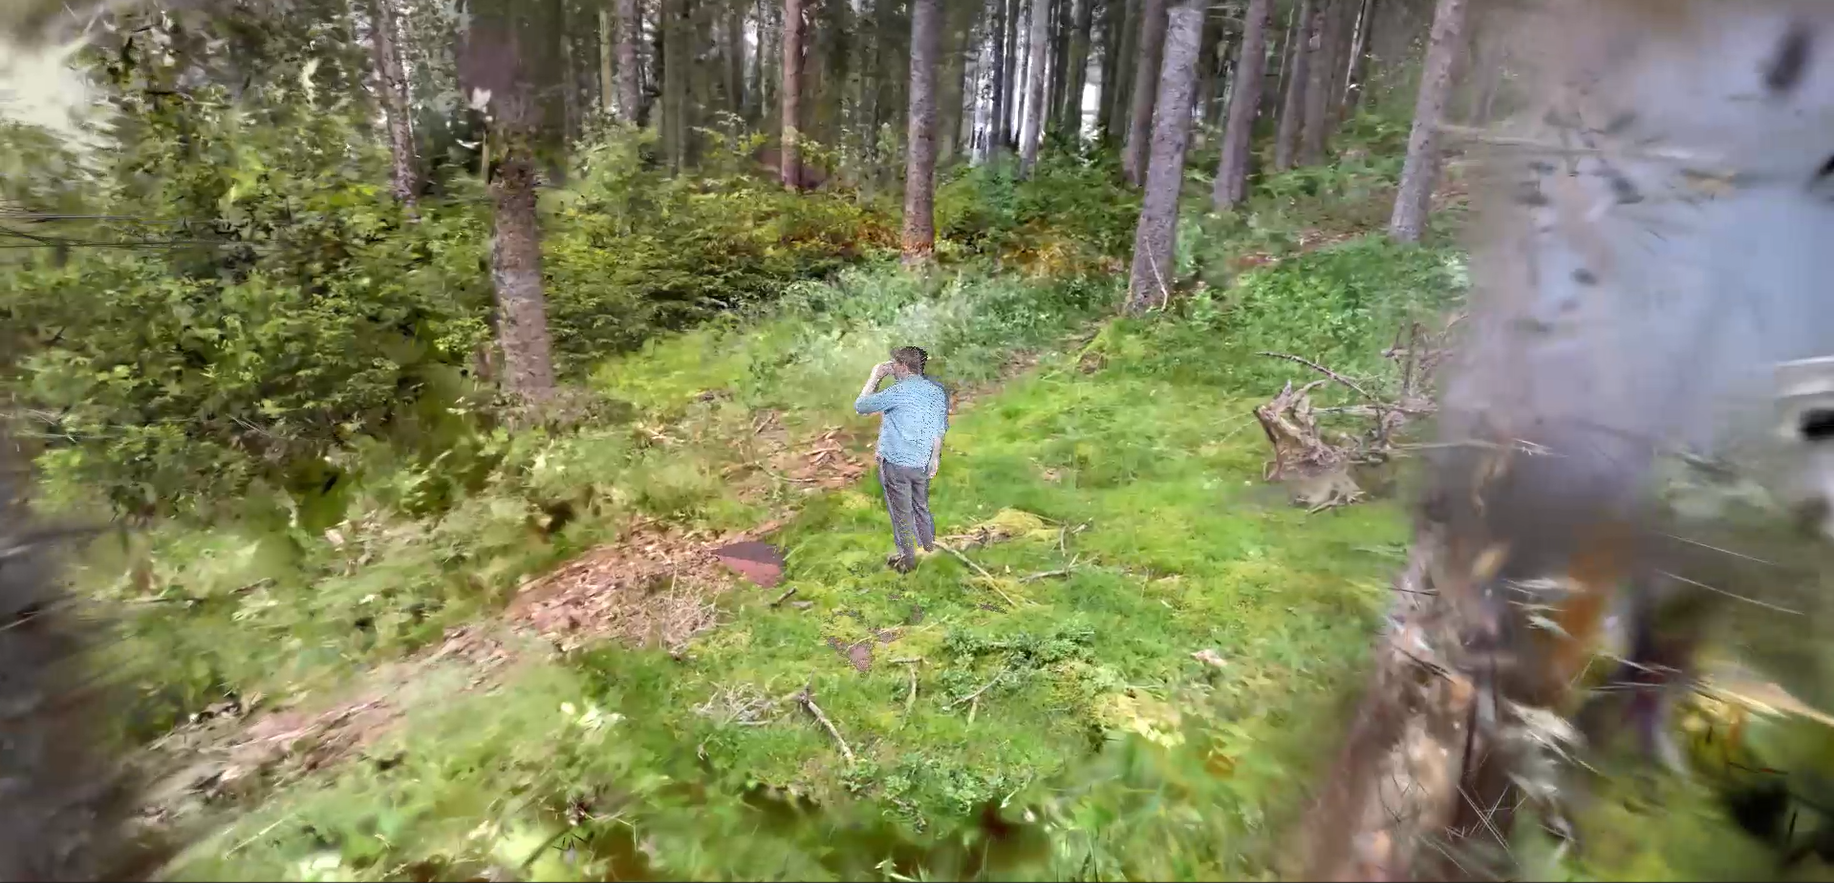
\includegraphics[width=\linewidth]{Pictures/ResPic2.png}
    \end{subfigure}
    \begin{subfigure}{.24\textwidth}
    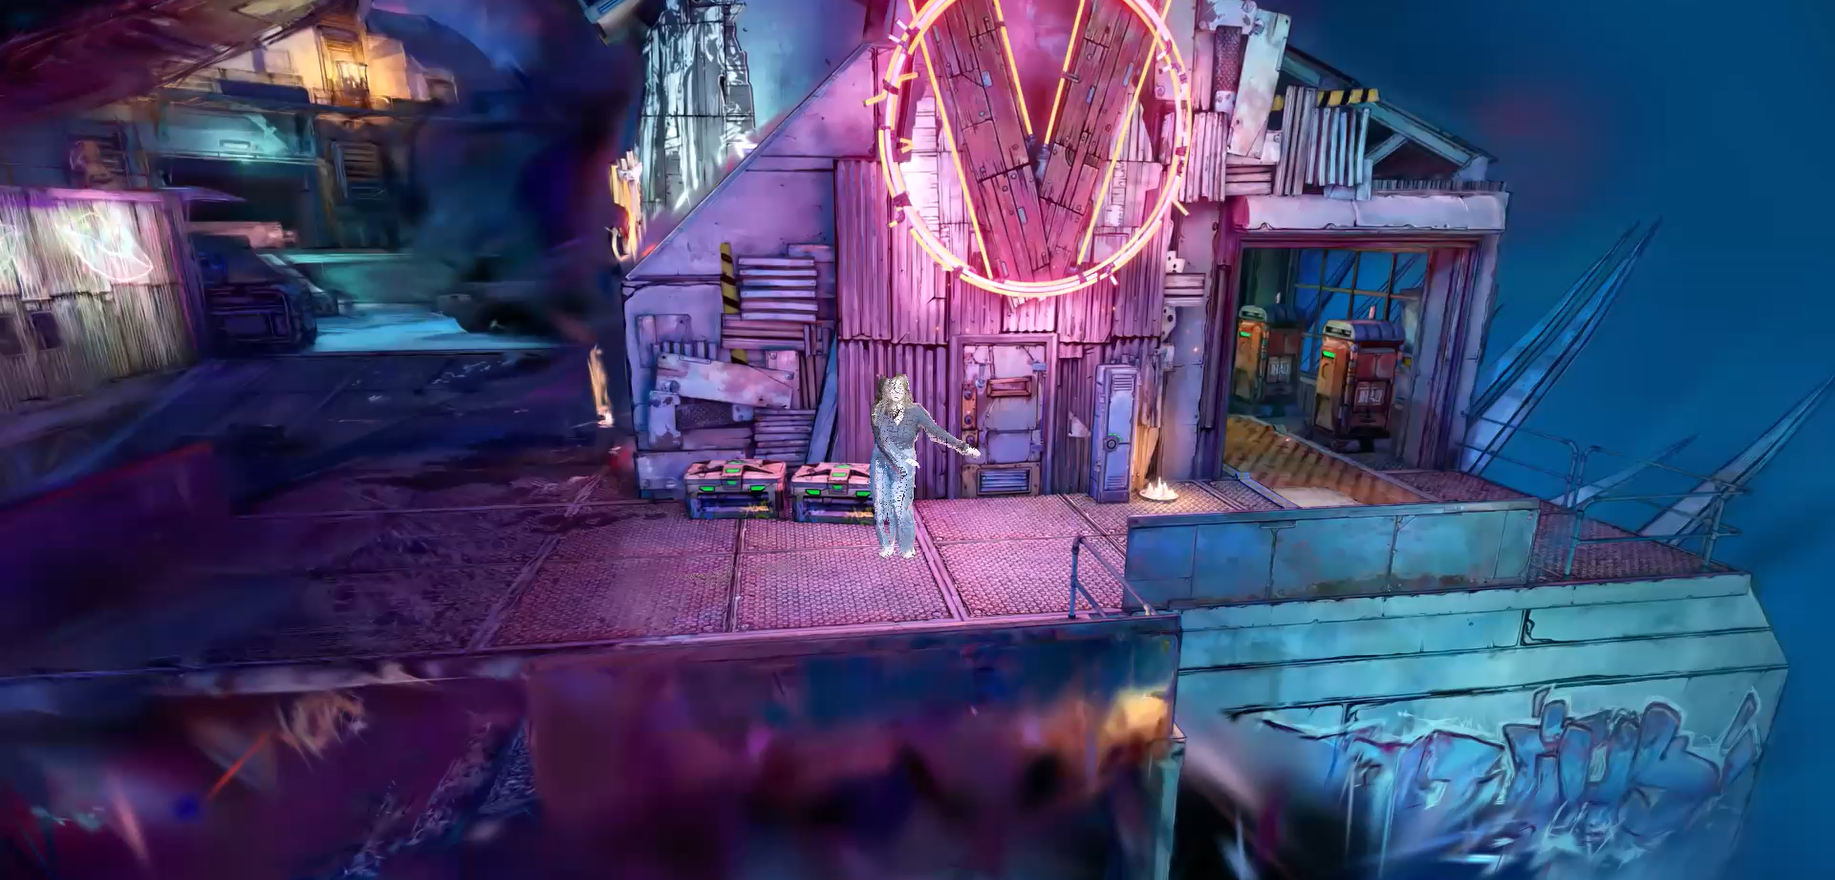
\includegraphics[width=\linewidth]{Pictures/ResPic3.png}
    \end{subfigure}
    \begin{subfigure}{.24\textwidth}
    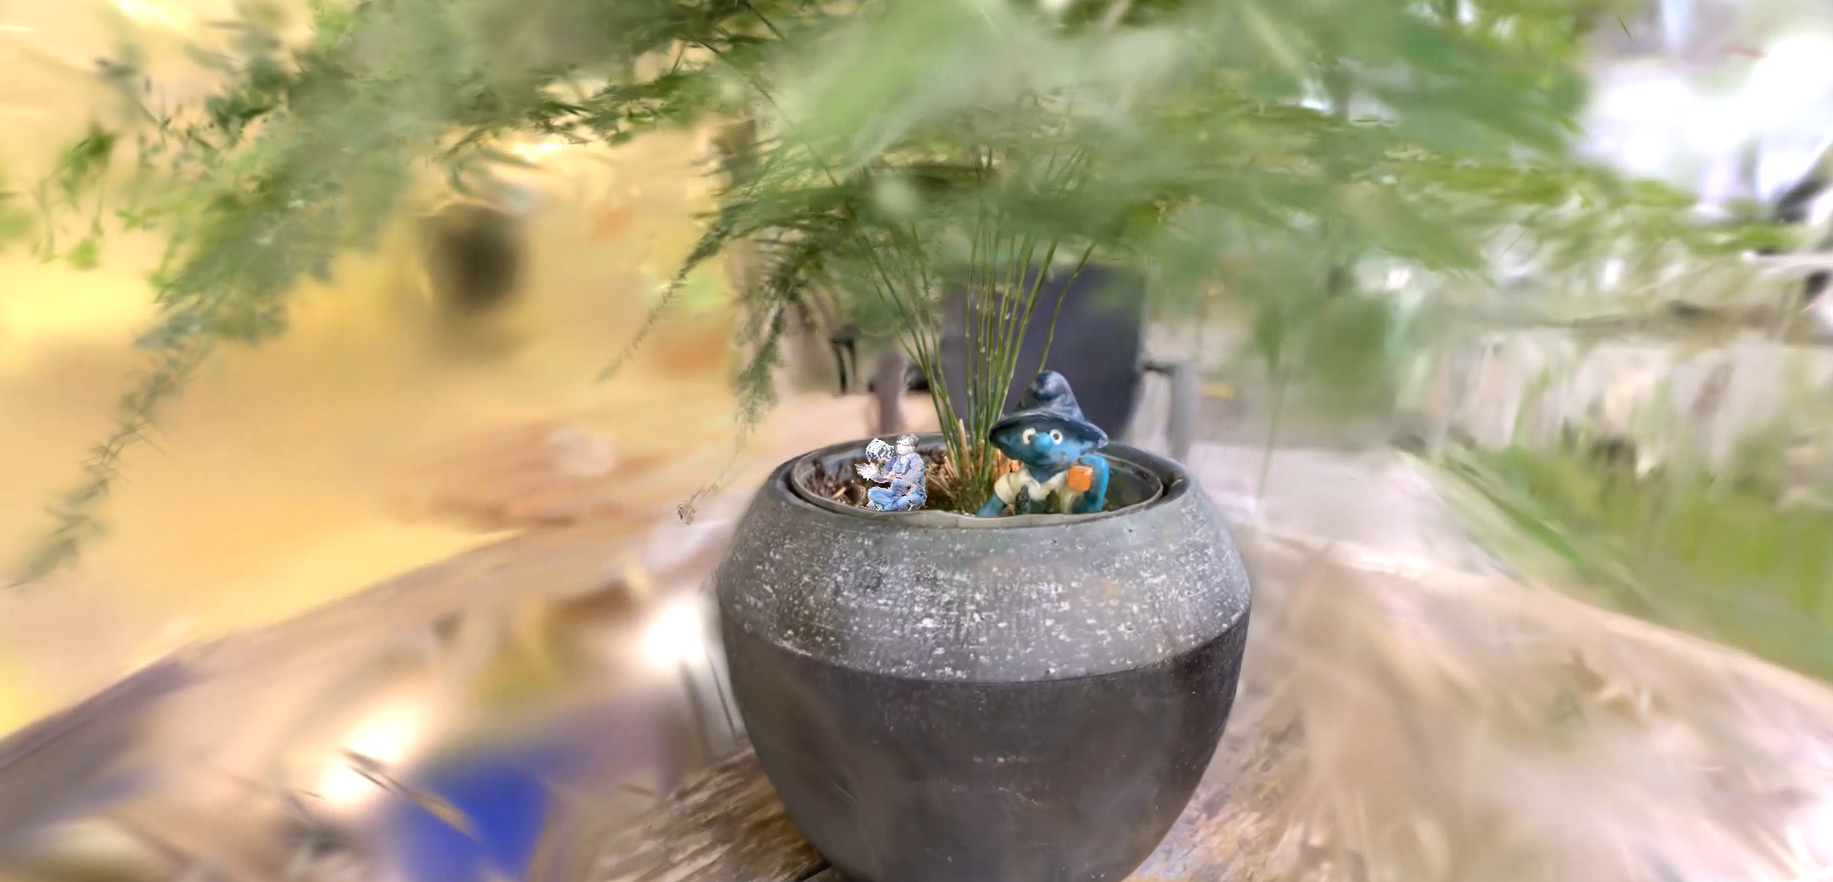
\includegraphics[width=\linewidth]{Pictures/ResPic4.png}
    \end{subfigure}
    \caption{Result Pictures out of Videos created at an Exhibition}
    \label{fig:ResultPictures}
\end{figure}
We were able to achieve the following results with our approach. It took two people seven minutes to set up the hardware. From setup to the point at which recordings could be made at a work show was achieved in approx. ninety minutes. The difference in time is largely due to lighting dependencies, camera properties of the Kinect and probably the USB-C connection.

At the exhibition where the setup was exhibited, over 30 short recordings were made, all of which were available to those filmed at six pm in the evening. The processing time of the five-second recordings was approx. six minutes.

Our project makes it possible to play “point cloud videos” in a game engine and combine them with a Gaussian Splat.

The best calibration results were achieved with the cameras at a distance of 1.5 meters to 2 meters from the calibration object. It was helpful not to have direct sunlight falling on the calibration object through a window.

In our work, we found that the ArUco cube produces more accurate calibration results than the ChArUco poster.

The post-processing method is quite unreliable. It often leads to errors where parts of the object in the center of the scene disappear or the center is completely removed. To circumvent this problem, the “Depth\_trunc” of Open3D for generating the point clouds from the depth images was often changed to achieve similar results as described above in the section on point cloud post processing.

\section{Conclusion}
Through our work, we were able to show a simple way to create visually convincing volumetric videos without a lot of equipment.  We were also able to identify ways in which this procedure can be improved.

Different calibration objects can be tested to improve the calibration. The ArUco cube delivered better results than the ChArUco board, which could be due to the size of the ArUco markers. At the same time, however, it could also be that the poster is more susceptible to direct light incidence and the light reflections make it more difficult for the tracking to be perceived. A good option for further testing could be to create a larger cube.

Post-processing to cut out the person or object in the center of the scene can be an uncertainty factor. This effect is particularly noticeable when people do not have their feet on the ground during the recording or are wearing black reflective shoes that cannot be detected by the Kinect. In our opinion, this section could be improved by working with masks or improving the post-processing process.

The visual quality of the point clouds in the final scene has a big difference to the static Gaussian splats that were generated. To reduce this difference, it would be possible to combine the data from the three Kinects with the Dynamic Gaussian Splatting project. In a series of tests conducted by our team, it has already been determined that three cameras might not be enough to achieve a very good visual result. However, an additional camera could already lead to an increase in quality.
It can also be evaluated in future work whether the data from Kinect cameras can be combined with the work of 4K4D. This could also lead to an increase in the quality of the result without increasing the hardware effort.

\section*{Translation Disclaimer}
The translation of the contents of this paper was carried out using DeepL. While efforts have been made to ensure accuracy, minor discrepancies or inaccuracies may be present. (DeepL SE, DeepL translator, 25.07.2024, https://www.deepl.com/de/translator).

\begin{thebibliography}{00}

\bibitem{b1}Bernhard Kerbl, Georgios Kopanas,Thomas Leimühler, and George Drettakis. 3D Gaussian Splatting for Real-Time Radiance Field Rendering, August 2023. arXiv:2308.04079 [cs].

\bibitem{b2} Jonathon Luiten, Georgios Kopanas, Bastian Leibe, and Deva Ramanan. Dynamic 3D Gaussians: Tracking by Persistent Dynamic View Synthesis, August 2023. arXiv:2308.09713 [cs].

\bibitem{b3} Haotong Lin, Sida Peng, Zhen Xu, Tao Xie, Xingyi He, Hujun Bao, and Xiaowei Zhou. Im4D: High-Fidelity and Real-Time Novel
View Synthesis for Dynamic Scenes, October 2023. arXiv:2310.08585 [cs].

\bibitem{b4} Ben Mildenhall, Pratul P. Srinivasan, Matthew Tancik, Jonathan T. Barron, Ravi Ramamoorthi, and Ren Ng. NeRF: Representing Scenes as Neural Radiance Fields for View Synthesis, August 2020. arXiv:2003.08934  [cs].

\bibitem{b5} Zhen Xu, Sida Peng, Haotong Lin, Guangzhao He, Jiaming Sun, Yujun Shen, Hujun Bao, and Xiaowei Zhou. 4K4D: RealTime 4D View Synthesis at 4K Resolution, October 2023. arXiv:2310.11448  [cs].

\bibitem{b6} Tancik, Matthew; Weber, Ethan; Ng, Evonne; Li, Ruilong; Yi, Brent; Wang, Terrance et al. (2023): Nerfstudio: A Modular Framework for Neural Radiance Field Development. Online verfügbar unter http://arxiv.org/pdf/2302.04264.

\bibitem{b7} Wang, Shuzhe; Leroy, Vincent; Cabon, Yohann; Chidlovskii, Boris; Revaud, Jerome (2023): DUSt3R: Geometric 3D Vision Made Easy. Online verfügbar unter http://arxiv.org/pdf/2312.14132.

\end{thebibliography}

\vspace{12pt}

\end{document}
